\section{Effects of relativity}

	\subsection{Velocity transformation}
		Consider two inertial frames of reference $S$ and $S'$ with relative velocity $v$ along the $xx'$-axes.
		\begin{figure}[h!]
			\centering
			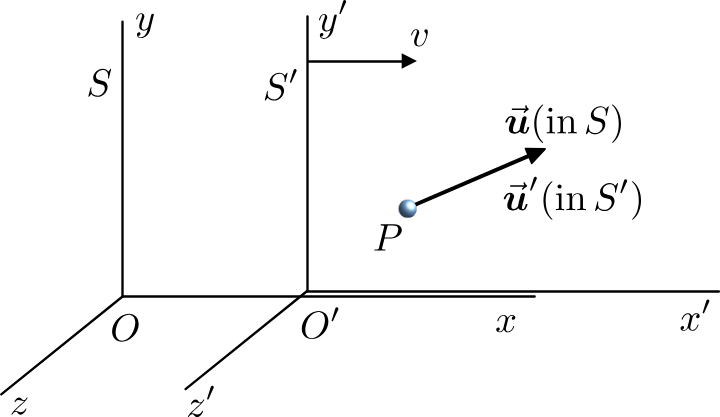
\includegraphics[width=0.45\textwidth]{figures/fig_velocity-transformation.png}
		\end{figure}
		Suppose a particle at $P$ is moving with a velocity $\vb{u}$ with respect to $S$ and with a velocity $\vb{u}'$ with respect to $S'$.
		
		Then the components of its velocity with respect to these two frames are as follows:
		\begin{align*}
			u_x=\dv{x}{t}\quad& u_y=\dv{y}{t}\quad u_z=\dv{z}{t} \\
			u_x'=\dv{x'}{t'}\quad& u_y'=\dv{y'}{t'}\quad u_z'=\dv{z'}{t'}
		\end{align*}
		
		Now, from the Lorentz transformation of coordinates from $S$ to $S'$, we have
		\begin{align*}
			x'&=\gamma\qty(x-\beta ct) \\
			\implies\dd{x'}&=\gamma\qty(\dd{x}-\beta c\dd{t}) \\
			\implies\dd{x'}&=\gamma\qty(\dd{x}-v\dd{t})
		\end{align*}
		Again
		\begin{align*}
			ct'&=\gamma\qty(ct-\beta x) \\
			\implies c\dd{t'}&=\gamma\qty(c\dd{t}-\beta\dd{x}) \\
			\implies\dd{t'}&=\gamma\qty(\dd{t}-\dfrac{\beta}{c}\dd{x})=\gamma\qty(\dd{t}-\dfrac{v/c}{c}\dd{x}) \\
			\implies\dd{t'}&=\gamma\qty(\dd{t}-\dfrac{v}{c^2}\dd{x})
		\end{align*}
		Finally,
		\begin{align*}
			\dd{y'}=\dd{y}\qq{and}\dd{z'}=\dd{z}
		\end{align*}
		
		Now, we obtain
		\begin{align*}
			u_x'=\dv{x'}{t'}&=\dfrac{\gamma\qty(\dd{x}-v\dd{t})}{\gamma\qty(\dd{t}-{v}/{c^2}\dd{x})} \\
				&=\dfrac{\dd{t}\qty(\dv*{x}{t}-v)}{\dd{t}\qty(1-v/c^2\cdot\dv*{x}{t})} \\
			\implies u_x'&=\dfrac{u_x-v}{1-u_xv/c^2}
		\end{align*}
		
		Likewise,
		\begin{align*}
			u_y'=\dv{y'}{t'}&=\dfrac{\dd{y}}{\gamma\qty(\dd{t}-{v}/{c^2}\dd{x})} \\
				&=\dfrac{\dv*{y}{t}}{\gamma\qty(\dd{t}-v/c^2\cdot\dv*{x}{t})} \\
			\implies u_y'&=\dfrac{u_y\sqrt{1-\beta^2}}{1-u_xv/c^2}
		\end{align*}
		
		Similarly,
		\begin{align*}
			u_z'&=\dfrac{u_z\sqrt{1-\beta^2}}{1-u_xv/c^2}
		\end{align*}
		
		Therefore, we obtain the \emph{Lorentz velocity transformation} equations as
		\begin{equation*}
			\boxed{
				\begin{aligned}
					u_x'&=\dfrac{u_x-v}{1-u_xv/c^2} \\
					u_y'&=\dfrac{u_y\sqrt{1-\beta^2}}{1-u_xv/c^2} \\
					u_z'&=\dfrac{u_z\sqrt{1-\beta^2}}{1-u_xv/c^2}
				\end{aligned}
			}
		\end{equation*}
		
		The \emph{inverse Lorentz velocity transformation} equations would then be
		\begin{equation*}
			\boxed{
				\begin{aligned}
					u_x&=\dfrac{u_x'+v}{1+u_x'v/c^2} \\
					u_y&=\dfrac{u_y'\sqrt{1-\beta^2}}{1+u_x'v/c^2} \\
					u_z&=\dfrac{u_z'\sqrt{1-\beta^2}}{1+u_x'v/c^2}
				\end{aligned}
			}
		\end{equation*}
		
		\textbf{Special case}: Suppose the motion of $P$ is along the $xx'$-axes, then we would have
		\begin{align*}
			u_x=u\quad u_y=0\quad u_z=0
		\end{align*}
		Then we would have $u_x'=u'$ and $u_y'=u_z'=0$. Then we obtain the forward and inverse Lorentz velocity transformations to be
		\begin{equation*}
			\boxed{
				u'=\dfrac{u-v}{1-uv/c^2}\qq{and}u=\dfrac{u'+v}{1+u'v/c^2}
			}
		\end{equation*}
		The above equations are referred to as \emph{Einstein's law of relativistic velocity addition}.